%% Template for a preprint Letter or Article for submission
%% to the journal Nature.
%% Written by Peter Czoschke, 26 February 2004
%%
\documentclass{nature}

%% make sure you have the nature.cls and naturemag.bst files where
%% LaTeX can find them
\bibliographystyle{naturemag}

\title{Optimal task allocation in systems with limited communication}

%% Notice placement of commas and superscripts and use of &
%% in the author list
\usepackage{amsthm}
\newtheorem{theorem}{Theorem}
\newtheorem{lemma}{Lemma}
\newtheorem{claim}{Claim}
\newtheorem{corollary}{Corollary}
\newtheorem{proposition}{Proposition}
\usepackage{amsmath}
\usepackage{amsfonts}
\usepackage{amssymb}
\usepackage{enumerate}
\usepackage{mathtools}

\DeclareMathOperator*{\argmin}{\arg\!\min\>}
\newcommand{\amin}[1]{\underset{#1}\argmin}
\DeclareMathOperator*{\argmax}{\arg\!\max\>}
\newcommand{\amax}[1]{\underset{#1}\argmax}
\DeclarePairedDelimiter\ceil{\lceil}{\rceil}
\DeclarePairedDelimiter\floor{\lfloor}{\rfloor}

\newcommand{\vnorm}[1]{\left|\left|#1\right|\right|}
\newcommand{\D}[2]{\frac{d#1}{d#2}}
\newcommand{\PD}[2]{\frac{\partial #1}{\partial #2}}
\newcommand{\V}[1]{\mathbf{#1}}
\newcommand{\ubar}[1]{\underline{#1}}

\def\a{\mathbf{a}}    % Action profile
\def\Z{\mathbb{Z}}    % Integers
\def\R{\mathbb{R}}    % Reals
\def\N{\mathcal{N}}   % Naturals
\def\td{\mathbf{t}}   % response-threshold value
\def\sig{\mathcal{S}} % Sigmoid function

\def\citerq{$^\text{citation reqd.}$}

\author{Anshul Kanakia$^{1,2}$, Nikolaus Correll$^{1,2}$ \& Behrouz Touri$^{1,3}$}


\begin{document}

\maketitle

\begin{affiliations}
 \item College of Engineering and Applied Sciences, University of Colorado, Boulder, USA. 
 \item Dept. of Computer Science.
 \item Dept. of Electrical, Computer \& Energy Engineering.
\end{affiliations}

\begin{abstract}
Task allocation in systems that are subject to communication constraints is ubiquitous in nature at all scales, ranging from cellular systems\cite{Yoshida2010, Suzuki2015} and social insects\cite{Robinson1987, Gordon1996, Bonabeau1998, Theraulaz1998} to large animal herds\cite{Conradt2003, Conradt2005} and human society\cite{Raafat2009}. Although the ability to communicate decisions such as voting\cite{Conradt2003} increases with agent complexity, inter-agent communication might not always possible. Formalizing such systems as a global game, a concept from the field of game theory, reveals that a simple threshold policy leads to a Bayesian Nash Equilibrium, that is an optimal assignment in the absence of communication between agents. While this result provides an hypothesis about the inner workings of a wide range of systems in which limited communication between agents is likely, it provides a formal explanation for threshold-based task allocation in social insects. In particular, we show how noise in perception in such systems leads to the observation of sigmoid response threshold functions, and how the resulting trade-off between exploration and exploitation\cite{Bonabeau1997} can be used to design engineered systems ranging from swarm robotics\cite{Martinoli1999, Krieger2000, Kube2000, Mataric2003, Gerkey2004} to smart composites\cite{McEvoy2015}. 
\end{abstract}

We are considering the following scenario. There are a group of individual agents attempting to perform some collaborative task. All agents observe a common stimulus of a certain magnitude associated with this task. Observation of this stimulus is subject to noise, and therefore subjective to each agent. Agents do not share any information. All agents decide, for themselves, whether or not to engage in the collaborative task. When a critical mass of agents willing to take part in the task is achieved, the task is successfully attempted, otherwise the attempt automatically fails. 

We have seen situations like this in a number of different fields including ethology\cite{Robinson1987, Gordon1996, Bonabeau1998, Theraulaz1998}, neurology\cite{Yoshida2010, Suzuki2015}, sociology \cite{Raafat2009}, economics\cite{Morris2000}, and robotics\cite{Martinoli1999, Krieger2000, Kube2000, Pynadath2002, Gerkey2003, Mataric2003, Gerkey2004, Kanakia2014}. While collaboration in social organisms has been a topic of study for centuries, the underlying mechanisms of this process still elude researchers\citerq. A broadening in thinking of the way division of labor is achieved in social insect colonies is discussed by Gordon\cite{Gordon1996}. Here, the idea that individuals in a swarm decide what task to perform using both internal and external triggers in a dynamically shifting environment is first cultivated. In contrast, prior models outlined by Gordon\cite{Gordon1996} first attributed task allocation mechanisms to innate physiological differences in individuals (such as age and size, in research from the 1960s/70s\cite{Michener1974, Oster1978}) while later models tended to focus heavily on external agent stimulus (such as pheromone levels, seen in research from the 1980s\cite{Robinson1987}). It is clear now that a combination of both internal and external parameters in essential for understanding the underlying mechanisms governing task-allocation in multi-agent systems.

This problem setup can be formulated as a \emph{global game}\cite{Carlsson1993}. A global game is game theoretic formulation where agents' utilities for taking an action depend not only on a shared underlying noisy signal, but also their imperfect beliefs of other agents' strategies. A classical example is a bank-run during a financial crisis\cite{Morris2000}. Here, agents engage in a bank-run based on their own, noisy, perception of the global financial situation as well as on their assessment how likely other players are to withdraw their savings. Although the classical global game assumes each agent to predict the other agents' behaviors, it turns out that agents can reach an equilibrium without this capacity\cite{Morris2000}, making this theory applicable to a much wider range of systems.

We formalize the task allocation problem description within the global game context to mathematically prove the existence of a Bayesian Nash Equilibrium (BNE) when threshold based strategies are used to solve the problem. Consider a set of $n$ agents and suppose that each agent has an action set $A_i=\{0,1\}$ where $0$ represents \emph{not participating} in the task and $1$ represents \emph{participating} in the task. Every agent is also aware of the total number of other agents, $n$ in the system. For the purposes of analysis we assume the decision to act or not act is made by all agents at the same time, i.e. this is a one-shot game with no notion of time. The \emph{magnitude} parameter $\tau$ of the given task also plays an important role in our formalism. We let $\tau$ be an (often random) real number which represents how many agents are required to complete a task. We further assume that it belongs to an interval $E=[c,d]$ in $\R$.  Finally, we let $u_i:A_i\times\Z^+\times \R\to \R$ be the utility of the $i^{\text{th}}$ agent, where $u_i(a_i,g,\tau)$ is the utility of the $i^{\text{th}}$ agent when $g$ other agents have decided to participate in the task of magnitude $\tau$. In general, the utility of each agent depends on the joint actions of the rest of the agents. However, here we assume that the utility depends only on the number of agents participating in the activity (The following discussions can be substantially generalized but this form of utility serves the purpose of this study). 

We define a task $T$ to be a \emph{concurrent benefit} task if:
\begin{enumerate}[a.]
	\item $u_i(1,g,\tau)-u_i(0,g,\tau)$ is an increasing and continuous function of $\tau$ for any $a_i\in A_i$ and $g$. We further assume that $|u_i(1,g,\tau)-u_i(0,g,\tau)|\leq \tau^p$ for some $p\geq 1$.
	\item For extreme magnitude ranges, taking part in the activity is either appealing or repelling, i.e.\ there exists $\underline{\tau},\bar{\tau}\in (c,d)$ with $\underline{\tau}\leq \bar{\tau}$ such that for any $\tau\geq \bar{\tau}$, we have $u_i(1,g,\tau)>u_i(0,g,\tau)$ and for $\tau\leq \underline{\tau}$, the only equilibrium of the game is $(0,0,\ldots,0)$. 
\end{enumerate}

Note that in order to have such a task, we need the above conditions to hold for all the agents, i.e.\ for all $i\in\{1,\ldots,n\}$. An example of a utility function that would satisfy such conditions is a function $u_i(a_i,g,\tau)=a_i(1-e^{-(g+1)}+\tau)$. In most real-world scenarios agents have a common utility function which is aligned with the system's objective but, in general, they may have different utility functions that need to satisfy the above conditions. 

\begin{figure}
	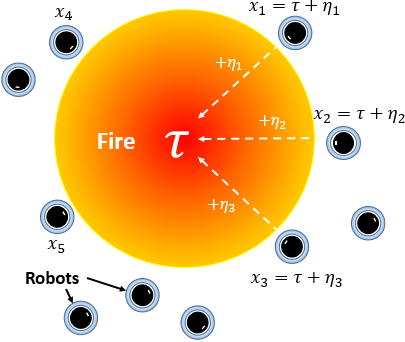
\includegraphics[width=0.5\columnwidth]{../figures/globalgamesetup.png}
	\caption{A multi-agent fire fighting scenario set up as a global game. Each player's imperfect estimate of the task is represented by $x_i$, a sum of the global magnitude parameter-$\tau$ and noisy sensor measurements-$\eta_i$.}\vspace{-10px}\label{fig:ggsetup}
\end{figure}

The main challenge in devising strategies in performing a concurrent benefit task is that the true value of $\tau$ is not easily accessible to the agents. For example, consider the firefighting scenario described above. The magnitude of the task is not easily estimated by each agent and they only have noisy, imperfect information through their on-board sensors and their local measurements.  We model this imperfect knowledge by assuming that agent $i$ observes $x_i=\tau+\eta_i$ where $\eta_i$ is a Gaussian $\mathcal{N}(0,\sigma_i^2)$ random variable, as seen in Fig.~\ref{fig:ggsetup}. Throughout our discussion, we assume that the task magnitude $\tau$ is a Gaussian random variable\footnote{This analysis is extendable to a larger class of random variables but for the simplicity of the discussion, we consider Gaussian random variables here.} and it is independent of $\eta_1,\ldots,\eta_n$. Now, the main question is that given a agent's private measurement $x_i$, what is a \emph{sensible strategy} to follow. 

We refer to a function that maps measurements (observations) to actions $A_i$ as a strategy. Mathematically, a strategy $s_i$ for the $i$th agent is a (measurable) function $s_i:\R\to A_i$. Strategy $s_i$ prescribes what action the $i$th agent should take given its own measurement $x_i$. Given this, consider a set of agents with strategies $s_1,\ldots,s_n$. Let us denote the strategies of the $n-1$ agents other than the $i$th agent by the vector $s_{-i}=(s_1,\ldots,s_{i-1},s_{i+1},\ldots,s_n)$.  We say that a strategy $s_i$ is a \emph{threshold strategy} if $s_i(x)=\text{step}(x, t_i)$, i.e.\ the step function with a jump from 0 to 1 at $t_i$. For the $i$th agent, we define the best-response $BR(s_{-i})$ (to the strategies of the other agents) to be a strategy $\tilde{s}$ that for any $x\in \R$:
\begin{align*}\label{eqn:BR}
BR(s_{-i})(x)&=\tilde{s}(x)=\amax{a_i\in A_i} E(u_i(a_i,g,\tau)\mid x_i=x)\\
&=\amax{a_i\in A_i} E(u_i(a_i,\sum_{j\not=i}s_j(x_j),\tau)\mid x_i=x),
\end{align*}
where $E(\cdot \mid x_i)$ is the conditional probability of $u_i$ given the $i$th agent's observation. Note that given $x_i$ and the strategies of the other agents $s_{-i}=(s_1,s_2,\ldots,s_{i-1},s_{i+1},\ldots,s_n)$, $\tau$, and $s_j(x_j)$ will be a random variable. In other words, given the $i$th agent's observation $x_i$, the observation of the other agents and hence, their actions would be random from the $i$th agent perspective.

Now, we are ready to define what we mean by a \emph{sensible strategy}. We say that a strategy profile $s=(s_1,\ldots,s_n)$ is sensible strategy, if it leads to a \emph{Bayesian Nash Equilibrium} (BNE) \cite{fudenberg1998theory}, given $s_i=BR(s_{-i})$ for all $i\in \{1,\ldots,n\}$. In other words, with the current strategies of the $n$ agents, no agent has the incentive to deviate from its current strategy.

We now show that any task with concurrent benefit admits a threshold strategy BNE. In other words, it is sufficient for the agents to follow a simple algorithm: 
\begin{enumerate}[(i)]
\item Compare your noisy measurement $x_i$ to a threshold value $\td_i$,
\item If the measurement is above $\td_i$ take part in the collaborative task, otherwise hold off. 
\end{enumerate}

In general, the existence of a BNE for a game is a questionable fact. Especially, once we impose additional constraints on the structure of strategies. However, in this case, we can show that there exists a sensible threshold policy for the class of tasks with concurrent benefits. To prove this, we show some intermediate results. 
\begin{lemma}\label{lemma:thresholdBR}
Let $s=(s_1,\ldots,s_n)$ be a strategy profile consisting of threshold strategies for a task with concurrent benefit. Let $\tilde{s}_i=BR(s_{-i})$. Then $\tilde{s}_i$ is a threshold policy. 
\end{lemma}

\begin{proof}
We first show that if for some observation $x_i=x$, we have $BR(s_{-i})(x)=\tilde{s}_i(x)=1$, then $\tilde{s}_i(y)=1$ for $y\geq x$. To show this,  we note that $P(x_j\geq \tau_j\mid x_i=x)$ is an increasing function of $x$ as $x_j-x_i$ is a normally distributed random variable. Therefore, using the monotone property of concurrent tasks and the fact that $x_i=\tau+\eta_i$, we conclude that:
\vspace{-5px}
\begin{align*}
&E(u_i(1,\sum_{j\not=i}s_j(x_j),\tau)\mid x_i=y)\\ 
&\qquad-E(u_i(0,\sum_{j\not=i}s_j(x_j),\tau)\mid x_i=y)\\ 
&>E(u_i(1,\sum_{j\not=i}s_j(x_j),\tau)\mid x_i=x)\\
&\qquad-E(u_i(0,\sum_{j\not=i}s_j(x_j),\tau)\mid x_i=x)\geq 0.
\end{align*}
Therefore $\tilde{s}_i(y)=1$. Similarly, if for some value of $x$, we have $\tilde{s}_i(x)=0$, then it follows that $\tilde{s}_i(y)=0$ for $y\leq x$. Therefore, $\tilde{s}_i$ would be a threshold policy.  
\end{proof}

Based on the above lemma, we can view the best-response of threshold strategies as a mapping from $\R^n$ to $\R^n$ that maps $n$ thresholds of the original strategies to $n$ thresholds of the best-response strategies. Denote this mapping by $L:\R^n\to\R^n$. The next step is to show that this mapping is a continuous mapping. 
\begin{lemma}\label{lemma:continuous}
The mapping $L$ that maps the threshold values of threshold strategies to the threshold values of the best-response strategies is a continuous mapping. 
\end{lemma}
\begin{proof}
Let $x_{-i}=(x_1,\ldots,x_{i-1},x_{i+1},\ldots,x_n)$ be the vector of observations of $n-1$ agents except the $i$th agent. Note that the vector $(x_{-i},\tau)$ given $x_i=x$ is a normally distributed random vector with some continuous density function $f_{x}(x_{-i},\tau)$. Now, let $\{\alpha(k)\}$ be a sequence in $\R^n$ that is converging to $\alpha\in\R^n$. Let $\{\beta(k)\}$ be the sequence of thresholds corresponding to the best-response strategy of the strategy with threshold vector $\alpha(k)$. Let $s$ be the threshold strategy corresponding to the threshold vector $\alpha$ and let $\alpha^*$ be the threshold policy corresponding to the $BR(\alpha)$. By the definition of the best-response strategy, $\beta_i(k)$ is a point where 
\begin{align*}
&\int_{\R^{n}}f_{\beta(k)}(z,t)\left(u_i(1,\sum_{j\not=i}u^{\alpha_j(k)}(x_j),\tau)\right.\\
&\qquad\left.-u_i(0,\sum_{j\not=i}u^{\alpha_j(k)}(x_j),\tau)\right)d(z\times t)=0.
\end{align*}
Using the fact that $f$ has a Gaussian distribution and is continuous on all its arguments and the fact that $|u_i(\cdot,\cdot,\tau)|\leq \tau^p$, by taking the limit $k\to\infty$ and the dominated convergence theorem \cite{folland2013real}:
\begin{align*}
&\int_{\R^{n}}f_{\beta}(z,t)(u_i(1,\sum_{j\not=i}u^{\alpha_j}(x_j),\tau)\\ 
&\qquad-u_i(0,\sum_{j\not=i}u^{\alpha(k)}(x_j),\tau))d(z\times t)=0,
\end{align*}
where $u^{r}$ is a threshold strategy with threshold $r$. Therefore, the $\lim_{k\to\infty}L(\alpha(k))=L(\alpha)$ for a sequence $\{\alpha(k)\}$ that is converging to $\alpha$.
\end{proof}
Finally, through Lemmas~\ref{lemma:thresholdBR} and \ref{lemma:continuous}, we are ready to prove our main result. 

\begin{theorem}\label{thrm:mainthrm}
For a concurrent task $T$, suppose that the magnitude parameter $\tau$ is a Gaussian random variable. Also, suppose that $x_i=\tau+\eta_i$ where $\eta_1,\ldots,\eta_n$ are independent Gaussian random variables. Then, there exists a strategy profile $s=(s_1,\ldots,s_n)$ of threshold policies that is a Bayesian Nash Equilibrium.
\end{theorem}
\begin{proof}
By Lemma~\ref{lemma:thresholdBR}, the best response of a threshold policy is a threshold policy and hence, it induces the mapping $L$ from the space of thresholds $\R^n$ to itself. Also, by Lemma~\ref{lemma:continuous}, this mapping is a continuous mapping. Now, if $t_i$ is a sufficiently large threshold, then the second property of the concurrent benefit tasks implies that the $\tilde{t}_i\leq t_i$ because a large enough measurement $x_i$ implies that agent $i$ itself should take part in the task. Similarly, for sufficiently low threshold $t_i$, we will have $\tilde{t}_i\geq t_i$. Therefore, the mapping $L$ maps a box $[a,b]^n$ to itself, where $a$ is a sufficiently small scalar and $b>a$ is a sufficiently large scalar. Since a box $[a,b]^n$ is a convex closed set, by the Brouwer's fix point theorem \cite{border1990fixed}, we have that there exists a vector of threshold values $\alpha^*$ such that $\alpha^*=L(\alpha^*)$ and hence, there exists a Bayesian Nash Equilibrium for a concurrent task $T$.
\end{proof}

We have therefore shown that a simple response threshold is sufficient to achieve a Bayes Nash Equilibrium, that is there is no other strategy that will, on average, improve an individual agents reward. This insight is consistent with phenomenological observations in social insects, which are believed to use response thresholds for coordination. For example, Robinson\cite{Robinson1987} provides first empirical evidence for hormone regulated response-threshold labor division in honey bees. A number of other ethology research groups subsequently show similar hormone regulation based task-allocation processes in ants and termites providing further evidence of the ubiquitous nature of the response-threshold process. Roboticists have started using these models to engineer swarm systems\cite{Krieger2000}. 
Bonabeau \cite{Bonabeau1996} introduces the \emph{fixed} response-threshold model for division of labor in social insects which is later extended to incorporate the notion of \emph{dynamic} response-thresholds for task-allocation which overcomes a number of issues with the fixed model \cite{Theraulaz1998}.

Yet, observations in ethology suggest sigmoid threshold function\cite{Bonabeau1996}. We argue that this behavior is a direct result of using a simple discrete threshold under the influence of perception noise. Indeed, one can show that a sigmoid threshold function therefore emerges if there is noise in observing the stimulus. When engineering a system, this noise can be controlled and enhanced using computation, allowing artificial agents to trade between exploitation and exploration. 

After showing that discrete thresholds indeed result in a BNE for systems in which agents do not directly communicate, we will now show how sensor noise at the individual level results in a continuous response-threshold phenomena that is prevalent in MAS and social insects. 

Suppose that all the agents share the same utility function $u(a_i,g,\tau)$ and also, assume that the observation noise of the $n$ agents ($\eta_1,\ldots,\eta_n$) are independent and identically distributed (i.i.d) $\mathcal{N}(0,\sigma^2)$ Gaussian random variables. Then, it is not hard to see that there exists a BNE with threshold strategies that have the same threshold value $\td$ (see  \cite{Morris2000}). Now, consider a realization of $\tau=\hat{\tau}$ and suppose that we have a large number of agents $n$ observing a noisy variation of $\hat{\tau}$. Take for example the case of fire-fighting agents, and let $\hat{\tau}$ be the magnitude (including type, intensity, area, etc.) of the fire. Then, since the observations of the $n$ agents are independent given the value of $\tau$, they will be distributed according to $\mathcal{N}(\hat{\tau},\sigma^2)$ (given the value of $\tau$). Now consider the relative number of agents taking part in the activity given the realized magnitude parameter $\hat{\tau}$ and denote it by 
\begin{equation}\label{eqn:Nrel}
	N_{rel}(\hat{\tau}):=\frac{\#\text{agents with }x_i\geq \td}{n}.
\end{equation}

Then, we have the following theorem.
\begin{theorem}\label{thrm:relativefrequency}
For the relative number of agents $N_{rel}(\hat{\tau})$, we have
\begin{equation}
\lim_{n\to\infty}N_{rel}(\hat{\tau})=\Phi(\frac{\hat{\tau}-\td}{\sigma^2})
\end{equation}
where $\Phi$ is the cumulative distribution function (cdf) of a standard Gaussian. 
\end{theorem}
\begin{proof}
Note that $N_{rel}(\hat{\tau})=\frac{\sum_{i=1}^n\mathbf{I}_{x_i\geq \td}}{n}$ where $\mathbf{I}_{\alpha\geq \beta}$ is the indicator function for $\alpha\geq \beta$. But note that for a given $\hat{\tau}$, $x_i$s are i.i.d.\ $\mathcal{N}(\hat{\tau},\sigma^2)$ random variables, and hence, $\mathbf{I}_{x_i\geq \td}$s are i.i.d.\ random variables with $E(\mathbf{I}_{x_i\geq \td})=\Phi(\frac{\hat{\tau}-\td}{\sigma^2})$. Therefore, by the Law of Large Numbers \cite{durrett2010}, it follows that:
\vspace{-5px}
\begin{align*}
\lim_{n\to\infty}N_{rel}(\hat{\tau})=\Phi(\frac{\hat{\tau}-\td}{\sigma^2}).
\end{align*}
\vspace{-5px}
\end{proof}

\begin{figure}
	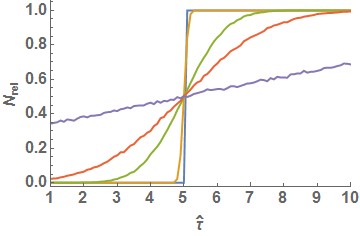
\includegraphics[width=.5\columnwidth]{../figures/thm2fig.png}
	\caption{Visualization of Theorem~\ref{thrm:relativefrequency} as $N_{rel}$ estimates $\Phi(\cdot)$. The plot was generated by running Eqn.~\ref{eqn:Nrel} 10,000 times for each point in $\hat{\tau} = [1,10,\text{ (inc.) }0.1]$. $n = 10$, $\td = 5$ and $x_i = \hat{\tau} + \eta_i$ ($\eta_i \sim\mathcal{N}(0, \sigma)$). Each curve in the plot is generated by sweeping $\sigma = \{0, 0.1, 1, 2, 10\}$, with $\sigma = 0$ being a step-function and $\sigma = 10$ having the \emph{flattest} slope.}\label{fig:thm2fig}
\end{figure}

Therefore, for large $n$, the relative frequency of agents taking part in the activity has a shape that follows the shape of the cdf of a standard Gaussian random variable, as seen in Fig.~\ref{fig:thm2fig}, i.e. agents may use deterministic threshold strategies but their aggregate behavior would appear to follow such a continues (sigmoid) threshold.

The final step to explain the prevalence of sigmoid functions in multiagent settings is to note that:
\begin{align*}
|\Phi(\frac{\hat{\tau}-\td}{\sigma^2})-\frac{1}{1+e^{-d(\frac{\hat{\tau}-\td}{\sigma^2})}}|\leq 0.01,
\end{align*}
for all $\hat{\tau}\in\R$ and some optimal value $d\approx 1.704$ (see \cite{camilli1994} and the references therein for the details of this approximation). This means that the aggregate behavior of the agents following deterministic threshold policies would (almost) follow the shape of a logistic sigmoid function whose drift is directly proportional to $\td$ and the slope  is inversely proportional to $\sigma^2$. 

%%% WHAT IS THE KEY PROBLEM WITH COLLABORATION? AGREEING ON WHEN TO DO IT REQUIRES A COMMON STIMULULUS AND COORDINATION

%%% THE PROBLEM HAS NOT ONLY BEEN STUDIED BY ETHOLOGISTS FOR ANTS BUT ALSO BY NEUROLOGISTS AND ECONOMISTS (GAME THEORY). WHO ELSE STUDIES TASK ALLOCATION IF IT IS REALLY SO IMPORTANT?

%%% WHAT ARE THE COMMONALITIES AMONG ALL THE CONSENSUS PROBLEMS / WHAT CLASS OF PROBLEMS ARE WE INTERESTED IN. THIS SHOULD MATCH THE GAME THEORY DEFINITION. THERE ARE MANY. WHERE HAS THE RESPONSE THRESHOLD ALREADY BEEN OBSERVED AND WHERE IS IT USED? ETHOLOGY AND ROBOTICS. THEY ARE DIFFERENT THAN WHAT GAME THEORY ASSUMES, HERE IS WHY: NOISE. 

% MAIN CLAIM: THERE ARE COUNTLESS SYSTMES THAT MUST USE RESPONSE THRESHOLDS, BECAUSE THEY ARE THE BEST WAY TO DO IT IN THIS CASE.

%Raafat et al. \cite{Raafat2009} discuss the underlying control mechanism for distributed coordination in a multi-agent system. They split the study of this mechanism into two levels; transmission-based and pattern-based control. 

%% Put the bibliography here, most people will use BiBTeX in
%% which case the environment below should be replaced with
%% the \bibliography{} command.
\bibliography{references}

\begin{addendum}
 \item Put acknowledgements here.
 \item[Competing Interests] The authors declare that they have no
competing financial interests.
 \item[Correspondence] Correspondence and requests for materials
should be addressed to Dr. Nikolaus Correll.~(email: nikolaus.correll@colorado.edu).
\end{addendum}

%%
%% TABLES
%%
%% If there are any tables, put them here.
%%

\end{document}
